% Options for packages loaded elsewhere
\PassOptionsToPackage{unicode}{hyperref}
\PassOptionsToPackage{hyphens}{url}
%
\documentclass[
  doc,floatsintext]{apa6}
\usepackage{amsmath,amssymb}
\usepackage{iftex}
\ifPDFTeX
  \usepackage[T1]{fontenc}
  \usepackage[utf8]{inputenc}
  \usepackage{textcomp} % provide euro and other symbols
\else % if luatex or xetex
  \usepackage{unicode-math} % this also loads fontspec
  \defaultfontfeatures{Scale=MatchLowercase}
  \defaultfontfeatures[\rmfamily]{Ligatures=TeX,Scale=1}
\fi
\usepackage{lmodern}
\ifPDFTeX\else
  % xetex/luatex font selection
\fi
% Use upquote if available, for straight quotes in verbatim environments
\IfFileExists{upquote.sty}{\usepackage{upquote}}{}
\IfFileExists{microtype.sty}{% use microtype if available
  \usepackage[]{microtype}
  \UseMicrotypeSet[protrusion]{basicmath} % disable protrusion for tt fonts
}{}
\makeatletter
\@ifundefined{KOMAClassName}{% if non-KOMA class
  \IfFileExists{parskip.sty}{%
    \usepackage{parskip}
  }{% else
    \setlength{\parindent}{0pt}
    \setlength{\parskip}{6pt plus 2pt minus 1pt}}
}{% if KOMA class
  \KOMAoptions{parskip=half}}
\makeatother
\usepackage{xcolor}
\usepackage{graphicx}
\makeatletter
\def\maxwidth{\ifdim\Gin@nat@width>\linewidth\linewidth\else\Gin@nat@width\fi}
\def\maxheight{\ifdim\Gin@nat@height>\textheight\textheight\else\Gin@nat@height\fi}
\makeatother
% Scale images if necessary, so that they will not overflow the page
% margins by default, and it is still possible to overwrite the defaults
% using explicit options in \includegraphics[width, height, ...]{}
\setkeys{Gin}{width=\maxwidth,height=\maxheight,keepaspectratio}
% Set default figure placement to htbp
\makeatletter
\def\fps@figure{htbp}
\makeatother
\setlength{\emergencystretch}{3em} % prevent overfull lines
\providecommand{\tightlist}{%
  \setlength{\itemsep}{0pt}\setlength{\parskip}{0pt}}
\setcounter{secnumdepth}{-\maxdimen} % remove section numbering
% Make \paragraph and \subparagraph free-standing
\ifx\paragraph\undefined\else
  \let\oldparagraph\paragraph
  \renewcommand{\paragraph}[1]{\oldparagraph{#1}\mbox{}}
\fi
\ifx\subparagraph\undefined\else
  \let\oldsubparagraph\subparagraph
  \renewcommand{\subparagraph}[1]{\oldsubparagraph{#1}\mbox{}}
\fi
\ifLuaTeX
\usepackage[bidi=basic]{babel}
\else
\usepackage[bidi=default]{babel}
\fi
\babelprovide[main,import]{english}
% get rid of language-specific shorthands (see #6817):
\let\LanguageShortHands\languageshorthands
\def\languageshorthands#1{}
% Manuscript styling
\usepackage{upgreek}
\captionsetup{font=singlespacing,justification=justified}

% Table formatting
\usepackage{longtable}
\usepackage{lscape}
% \usepackage[counterclockwise]{rotating}   % Landscape page setup for large tables
\usepackage{multirow}		% Table styling
\usepackage{tabularx}		% Control Column width
\usepackage[flushleft]{threeparttable}	% Allows for three part tables with a specified notes section
\usepackage{threeparttablex}            % Lets threeparttable work with longtable

% Create new environments so endfloat can handle them
% \newenvironment{ltable}
%   {\begin{landscape}\centering\begin{threeparttable}}
%   {\end{threeparttable}\end{landscape}}
\newenvironment{lltable}{\begin{landscape}\centering\begin{ThreePartTable}}{\end{ThreePartTable}\end{landscape}}

% Enables adjusting longtable caption width to table width
% Solution found at http://golatex.de/longtable-mit-caption-so-breit-wie-die-tabelle-t15767.html
\makeatletter
\newcommand\LastLTentrywidth{1em}
\newlength\longtablewidth
\setlength{\longtablewidth}{1in}
\newcommand{\getlongtablewidth}{\begingroup \ifcsname LT@\roman{LT@tables}\endcsname \global\longtablewidth=0pt \renewcommand{\LT@entry}[2]{\global\advance\longtablewidth by ##2\relax\gdef\LastLTentrywidth{##2}}\@nameuse{LT@\roman{LT@tables}} \fi \endgroup}

% \setlength{\parindent}{0.5in}
% \setlength{\parskip}{0pt plus 0pt minus 0pt}

% Overwrite redefinition of paragraph and subparagraph by the default LaTeX template
% See https://github.com/crsh/papaja/issues/292
\makeatletter
\renewcommand{\paragraph}{\@startsection{paragraph}{4}{\parindent}%
  {0\baselineskip \@plus 0.2ex \@minus 0.2ex}%
  {-1em}%
  {\normalfont\normalsize\bfseries\itshape\typesectitle}}

\renewcommand{\subparagraph}[1]{\@startsection{subparagraph}{5}{1em}%
  {0\baselineskip \@plus 0.2ex \@minus 0.2ex}%
  {-\z@\relax}%
  {\normalfont\normalsize\itshape\hspace{\parindent}{#1}\textit{\addperi}}{\relax}}
\makeatother

% \usepackage{etoolbox}
\makeatletter
\patchcmd{\HyOrg@maketitle}
  {\section{\normalfont\normalsize\abstractname}}
  {\section*{\normalfont\normalsize\abstractname}}
  {}{\typeout{Failed to patch abstract.}}
\patchcmd{\HyOrg@maketitle}
  {\section{\protect\normalfont{\@title}}}
  {\section*{\protect\normalfont{\@title}}}
  {}{\typeout{Failed to patch title.}}
\makeatother

\usepackage{xpatch}
\makeatletter
\xapptocmd\appendix
  {\xapptocmd\section
    {\addcontentsline{toc}{section}{\appendixname\ifoneappendix\else~\theappendix\fi\\: #1}}
    {}{\InnerPatchFailed}%
  }
{}{\PatchFailed}
\usepackage{csquotes}
\usepackage{orcidlink}
\usepackage[justification=Centering,position=top]{subfig}
\usepackage{caption}
\captionsetup[figure]{font=footnotesize}
\ifLuaTeX
  \usepackage{selnolig}  % disable illegal ligatures
\fi
\IfFileExists{bookmark.sty}{\usepackage{bookmark}}{\usepackage{hyperref}}
\IfFileExists{xurl.sty}{\usepackage{xurl}}{} % add URL line breaks if available
\urlstyle{same}
\hypersetup{
  pdftitle={Supplementary materials: Social influences on similarity judgments and intertemporal choice},
  pdfauthor={Francine W. Goh1 \& Jeffrey R. Stevens1},
  pdflang={en-EN},
  hidelinks,
  pdfcreator={LaTeX via pandoc}}

\title{Supplementary materials: Social influences on similarity judgments and intertemporal choice}
\author{Francine W. Goh\textsuperscript{1} \& Jeffrey R. Stevens\textsuperscript{1}}
\date{}


\shorttitle{Supplementary materials}

\authornote{

Francine W. Goh, \orcidlink{0000-0002-7364-4398} \url{https://orcid.org/0000-0002-7364-4398}.

Jeffrey R. Stevens, \orcidlink{0000-0003-2375-1360} \url{https://orcid.org/0000-0003-2375-1360}.

Department of Psychology, Center for Brain, Biology and Behavior, University of Nebraska-Lincoln, Lincoln, Nebraska, USA.

Correspondence concerning this article should be addressed to Jeffrey R. Stevens, B83 East Stadium, University of Nebraska-Lincoln, Lincoln, Nebraska, 68588. E-mail: \href{mailto:jeffrey.r.stevens@gmail.com}{\nolinkurl{jeffrey.r.stevens@gmail.com}}

}

\affiliation{\vspace{0.5cm}\textsuperscript{1} University of Nebraska-Lincoln}

\begin{document}
\maketitle

\renewcommand{\thetable}{S\arabic{table}}
\setcounter{table}{0}
\renewcommand{\thefigure}{S\arabic{figure}}
\setcounter{figure}{0}
\setcounter{page}{1}

\newpage

\begin{table}[tbp]

\begin{center}
\begin{threeparttable}

\caption{\label{tab:unnamed-chunk-1}Participant demographic information}

\small{

\begin{tabular}{lccc}
\toprule
 & \multicolumn{2}{c}{} \\
\cmidrule(r){2-4}
 & Study 1 & Study 2 & Study 3\\
\midrule
Gender &  &  & \\
\ \ \ Women & 43 & 63 & 47\\
\ \ \ Men & 26 & 22 & 16\\
\ \ \ Other & 0 & 1 & 2\\
Ethnicity &  &  & \\
\ \ \ American Indian/Alaskan Native & 0 & 0 & 0\\
\ \ \ Asian & 5 & 7 & 2\\
\ \ \ Black/African American & 3 & 1 & 2\\
\ \ \ Hispanic & 3 & 8 & 5\\
\ \ \ Latino & 0 & 1 & 0\\
\ \ \ Middle Eastern & 0 & 3 & 2\\
\ \ \ White/European American & 57 & 66 & 46\\
\ \ \ Biracial/Multiracial & 1 & 0 & 8\\
\bottomrule
\addlinespace
\end{tabular}

}

\begin{tablenotes}[para]
\normalsize{\textit{Note.} Table used with permission under a CC-BY4.0 license: Goh \& Stevens (2022); available at https://doi.org/10.31234/osf.io/xz68b}
\end{tablenotes}

\end{threeparttable}
\end{center}

\end{table}

\clearpage

\begin{table}[tbp]

\begin{center}
\begin{threeparttable}

\caption{\label{tab:unnamed-chunk-2}Number pairs for amount and delay similarity judgments for study 1}

\small{

\begin{tabular}{cc}
\toprule
Small value & \multicolumn{1}{c}{Large value}\\
\midrule
4 & 8\\
5 & 11\\
5 & 12\\
6 & 12\\
6 & 13\\
7 & 12\\
10 & 15\\
11 & 17\\
11 & 18\\
12 & 18\\
12 & 19\\
13 & 18\\
16 & 21\\
17 & 23\\
17 & 24\\
18 & 24\\
18 & 25\\
19 & 24\\
22 & 27\\
23 & 29\\
23 & 30\\
24 & 30\\
24 & 31\\
25 & 30\\
29 & 35\\
29 & 36\\
30 & 36\\
30 & 37\\
35 & 41\\
35 & 42\\
36 & 42\\
36 & 43\\
41 & 47\\
41 & 48\\
42 & 48\\
42 & 49\\
47 & 53\\
47 & 54\\
48 & 54\\
48 & 55\\
\bottomrule
\addlinespace
\end{tabular}

}

\begin{tablenotes}[para]
\normalsize{\textit{Note.} Table used with permission under a CC-BY4.0 license: Goh \& Stevens (2022); available at https://doi.org/10.31234/osf.io/xz68b}
\end{tablenotes}

\end{threeparttable}
\end{center}

\end{table}

\clearpage

\begin{center}
\begin{ThreePartTable}

\begin{TableNotes}[para]
\normalsize{\textit{Note.} Table used with permission under a CC-BY4.0 license: Goh \& Stevens (2022); available at https://doi.org/10.31234/osf.io/xz68b}
\end{TableNotes}

\small{

\begin{longtable}{cccc}\noalign{\getlongtablewidth\global\LTcapwidth=\longtablewidth}
\caption{\label{tab:unnamed-chunk-3}Intertemporal choice questions for study 1}\\
\toprule
Small amount & \multicolumn{1}{c}{Large amount} & \multicolumn{1}{c}{Short delay} & \multicolumn{1}{c}{Long delay}\\
\midrule
\endfirsthead
\caption*{\normalfont{Table \ref{tab:unnamed-chunk-3} continued}}\\
\toprule
Small amount & \multicolumn{1}{c}{Large amount} & \multicolumn{1}{c}{Short delay} & \multicolumn{1}{c}{Long delay}\\
\midrule
\endhead
4 & 8 & 17 & 23\\
4 & 8 & 17 & 24\\
4 & 8 & 18 & 24\\
4 & 8 & 18 & 25\\
5 & 11 & 10 & 15\\
5 & 12 & 10 & 15\\
6 & 12 & 10 & 15\\
6 & 13 & 10 & 15\\
7 & 12 & 47 & 53\\
7 & 12 & 47 & 54\\
7 & 12 & 48 & 54\\
7 & 12 & 48 & 55\\
10 & 15 & 23 & 29\\
10 & 15 & 23 & 30\\
10 & 15 & 24 & 30\\
10 & 15 & 24 & 31\\
11 & 17 & 4 & 8\\
11 & 18 & 4 & 8\\
12 & 18 & 4 & 8\\
12 & 19 & 4 & 8\\
13 & 18 & 29 & 35\\
13 & 18 & 29 & 36\\
13 & 18 & 30 & 36\\
13 & 18 & 30 & 37\\
16 & 21 & 5 & 11\\
16 & 21 & 5 & 12\\
16 & 21 & 6 & 12\\
16 & 21 & 6 & 13\\
17 & 23 & 7 & 12\\
17 & 24 & 7 & 12\\
18 & 24 & 7 & 12\\
18 & 25 & 7 & 12\\
19 & 24 & 11 & 17\\
19 & 24 & 11 & 18\\
19 & 24 & 12 & 18\\
19 & 24 & 12 & 19\\
22 & 27 & 41 & 47\\
22 & 27 & 41 & 48\\
22 & 27 & 42 & 48\\
22 & 27 & 42 & 49\\
23 & 29 & 13 & 18\\
23 & 30 & 13 & 18\\
24 & 30 & 13 & 18\\
24 & 31 & 13 & 18\\
25 & 30 & 35 & 41\\
25 & 30 & 35 & 42\\
25 & 30 & 36 & 42\\
25 & 30 & 36 & 43\\
29 & 35 & 25 & 30\\
29 & 36 & 25 & 30\\
30 & 36 & 25 & 30\\
30 & 37 & 25 & 30\\
35 & 41 & 16 & 21\\
35 & 42 & 16 & 21\\
36 & 42 & 16 & 21\\
36 & 43 & 16 & 21\\
41 & 47 & 19 & 24\\
41 & 48 & 19 & 24\\
42 & 48 & 19 & 24\\
42 & 49 & 19 & 24\\
47 & 53 & 22 & 27\\
47 & 54 & 22 & 27\\
48 & 54 & 22 & 27\\
48 & 55 & 22 & 27\\
\bottomrule
\addlinespace
\insertTableNotes
\end{longtable}

}

\end{ThreePartTable}
\end{center}

\clearpage

\begin{table}[tbp]

\begin{center}
\begin{threeparttable}

\caption{\label{tab:unnamed-chunk-4}Bayes factor interpretations according to Wagenmakers et al. (2018)}

\begin{tabular}{ll}
\toprule
Bayes factor & \multicolumn{1}{c}{Interpretation}\\
\midrule
> 100 & Extreme evidence for H$_{1}$\\
30 - 100 & Very strong evidence for H$_{1}$\\
10 - 30 & Strong evidence for H$_{1}$\\
3 - 10 & Moderate evidence for H$_{1}$\\
1 - 3 & Anecdotal evidence for H$_{1}$\\
1/3 - 1 & Anecdotal evidence for H$_{0}$\\
1/10 - 1/3 & Moderate evidence for H$_{0}$\\
1/30 - 1/10 & Strong evidence for H$_{0}$\\
1/100 - 1/30 & Very strong evidence for H$_{0}$\\
< 1/100 & Extreme evidence for H$_{0}$\\
\bottomrule
\addlinespace
\end{tabular}

\begin{tablenotes}[para]
\normalsize{\textit{Note.} Table used with permission under a CC-BY4.0 license: Goh \& Stevens (2022); available at https://doi.org/10.31234/osf.io/xz68b}
\end{tablenotes}

\end{threeparttable}
\end{center}

\end{table}

\clearpage



\begin{figure}

{\centering 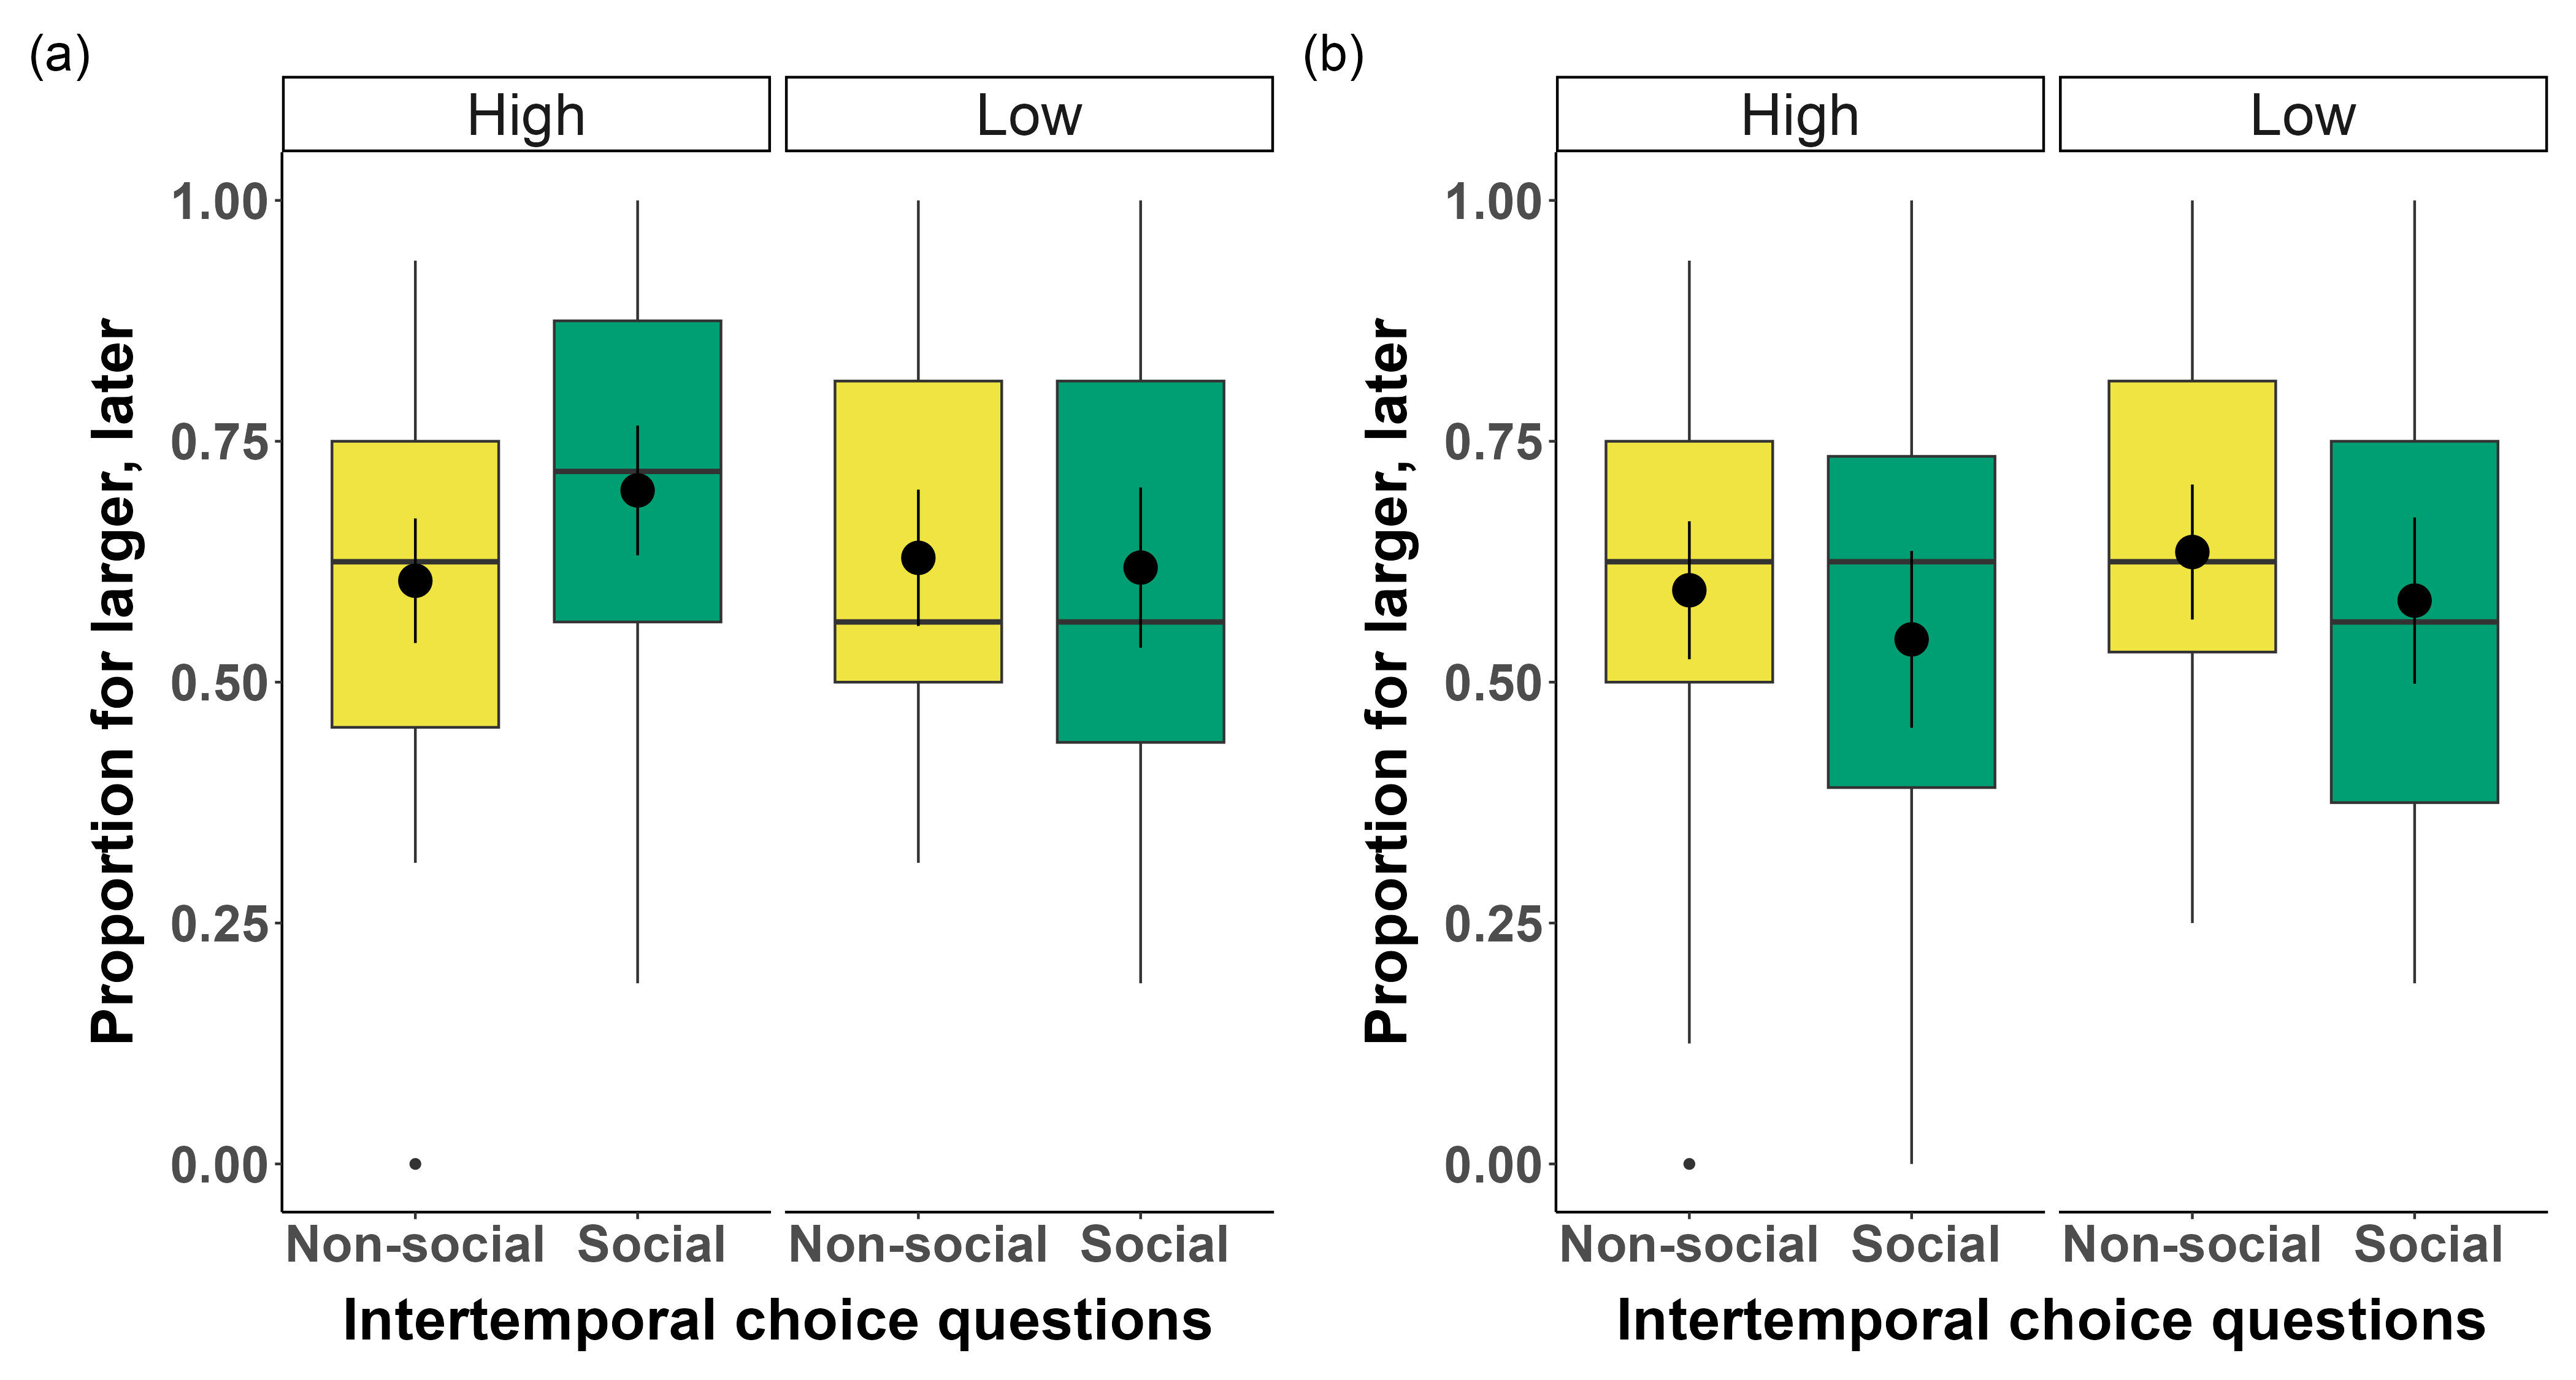
\includegraphics[width=1\linewidth]{figures/suggestibility_itc_1} 

}

\caption{Proportion of participant choices for the larger, later option for the (a) amount-focused and (b) delay-focused social information conditions for study 1. The left panels represent participant choices for the larger, later option for non-social compared to social intertemporal choice questions for those in the high suggestibility group while the right panels represent the comparison of these choices for participants in the low suggestibility group. Dots and error bars represent mean values and 95\% within-subject confidence intervals respectively. For boxplots, horizontal bars represent medians, boxes represent interquartile ranges (25\textsuperscript{th} - 75\textsuperscript{th} percentile), and whiskers represent 1.5 times the interquartile range. Figure used with permission under a CC-BY4.0 license: Goh \& Stevens (2022); available at \url{https://doi.org/10.31234/osf.io/xz68b}}\label{fig:suggestibility1}
\end{figure}



\begin{figure}
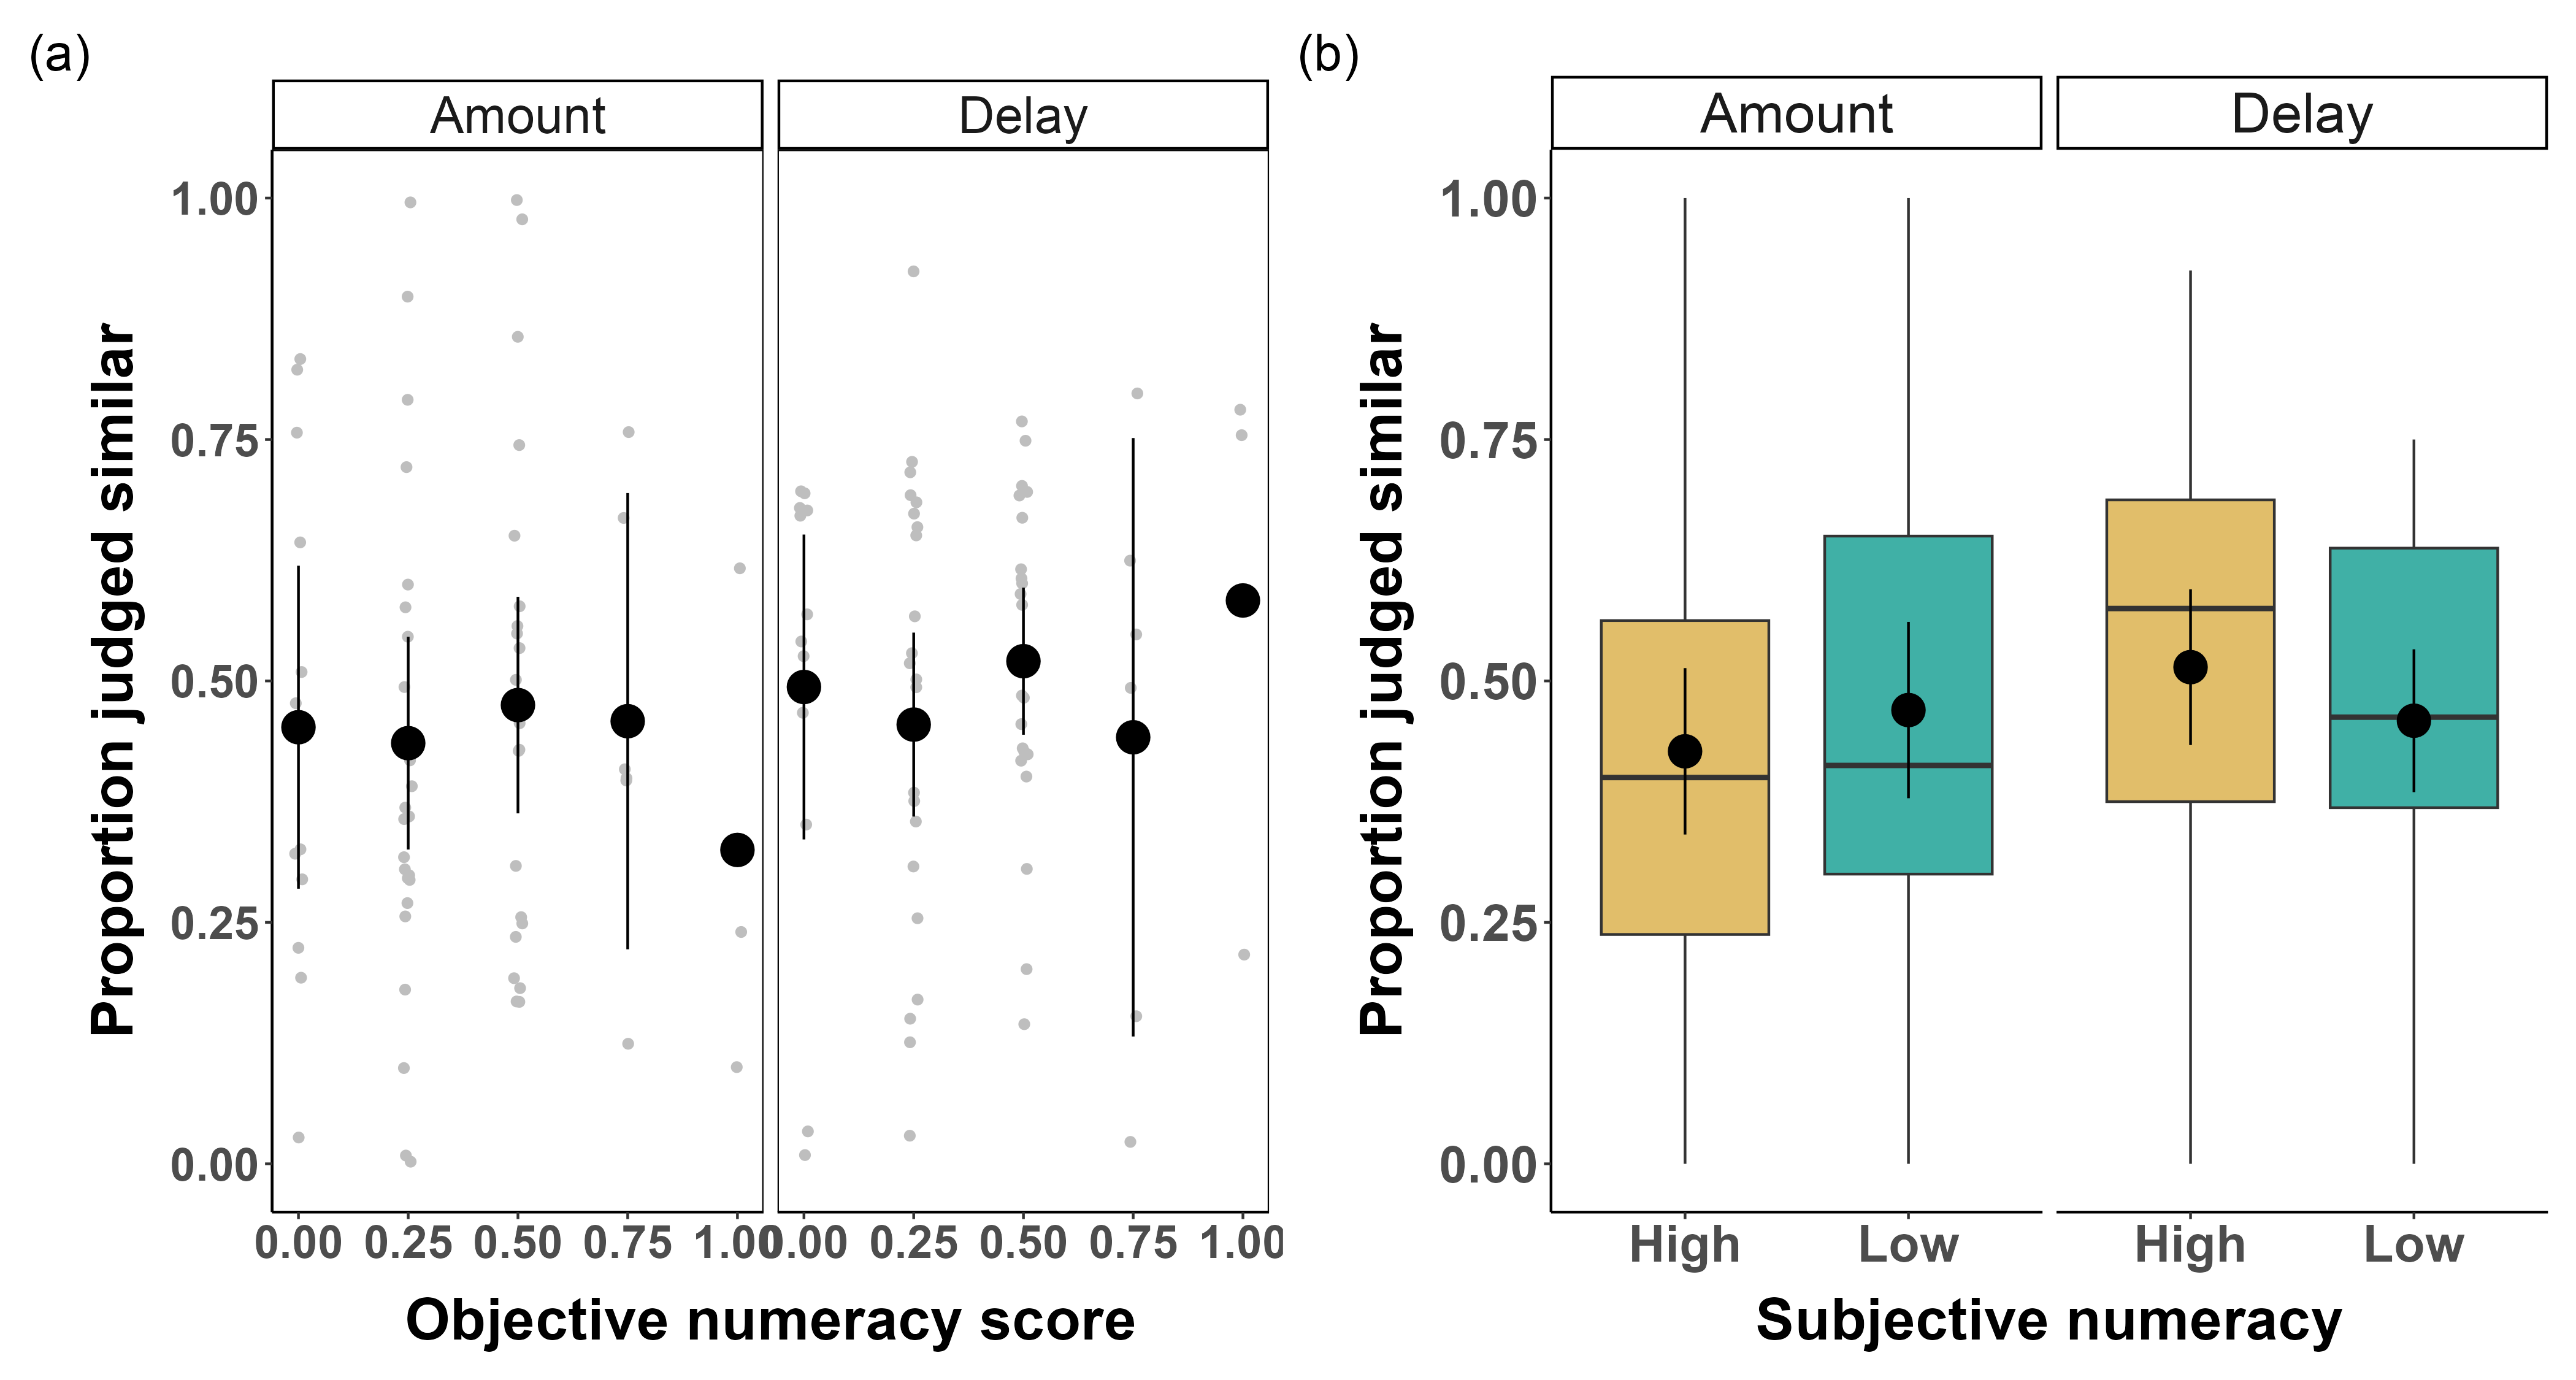
\includegraphics[width=1\linewidth]{figures/numeracy_judgments_1} \caption{Proportion of number pairs judged similar by participants according to (a) objective numeracy scores and (b) subjective numeracy levels for study 1. The left panels represent judgments in the amount similarity judgment task and the right panels represent judgments in the delay similarity judgment task. Dots and error bars represent mean values and 95\% within-subject confidence intervals respectively. For boxplots, horizontal bars represent medians, boxes represent interquartile ranges (25\textsuperscript{th} - 75\textsuperscript{th} percentile), and whiskers represent 1.5 times the interquartile range. Figure used with permission under a CC-BY4.0 license: Goh \& Stevens (2022); available at \url{https://doi.org/10.31234/osf.io/xz68b}}\label{fig:numeracyjudgments1}
\end{figure}



\begin{figure}
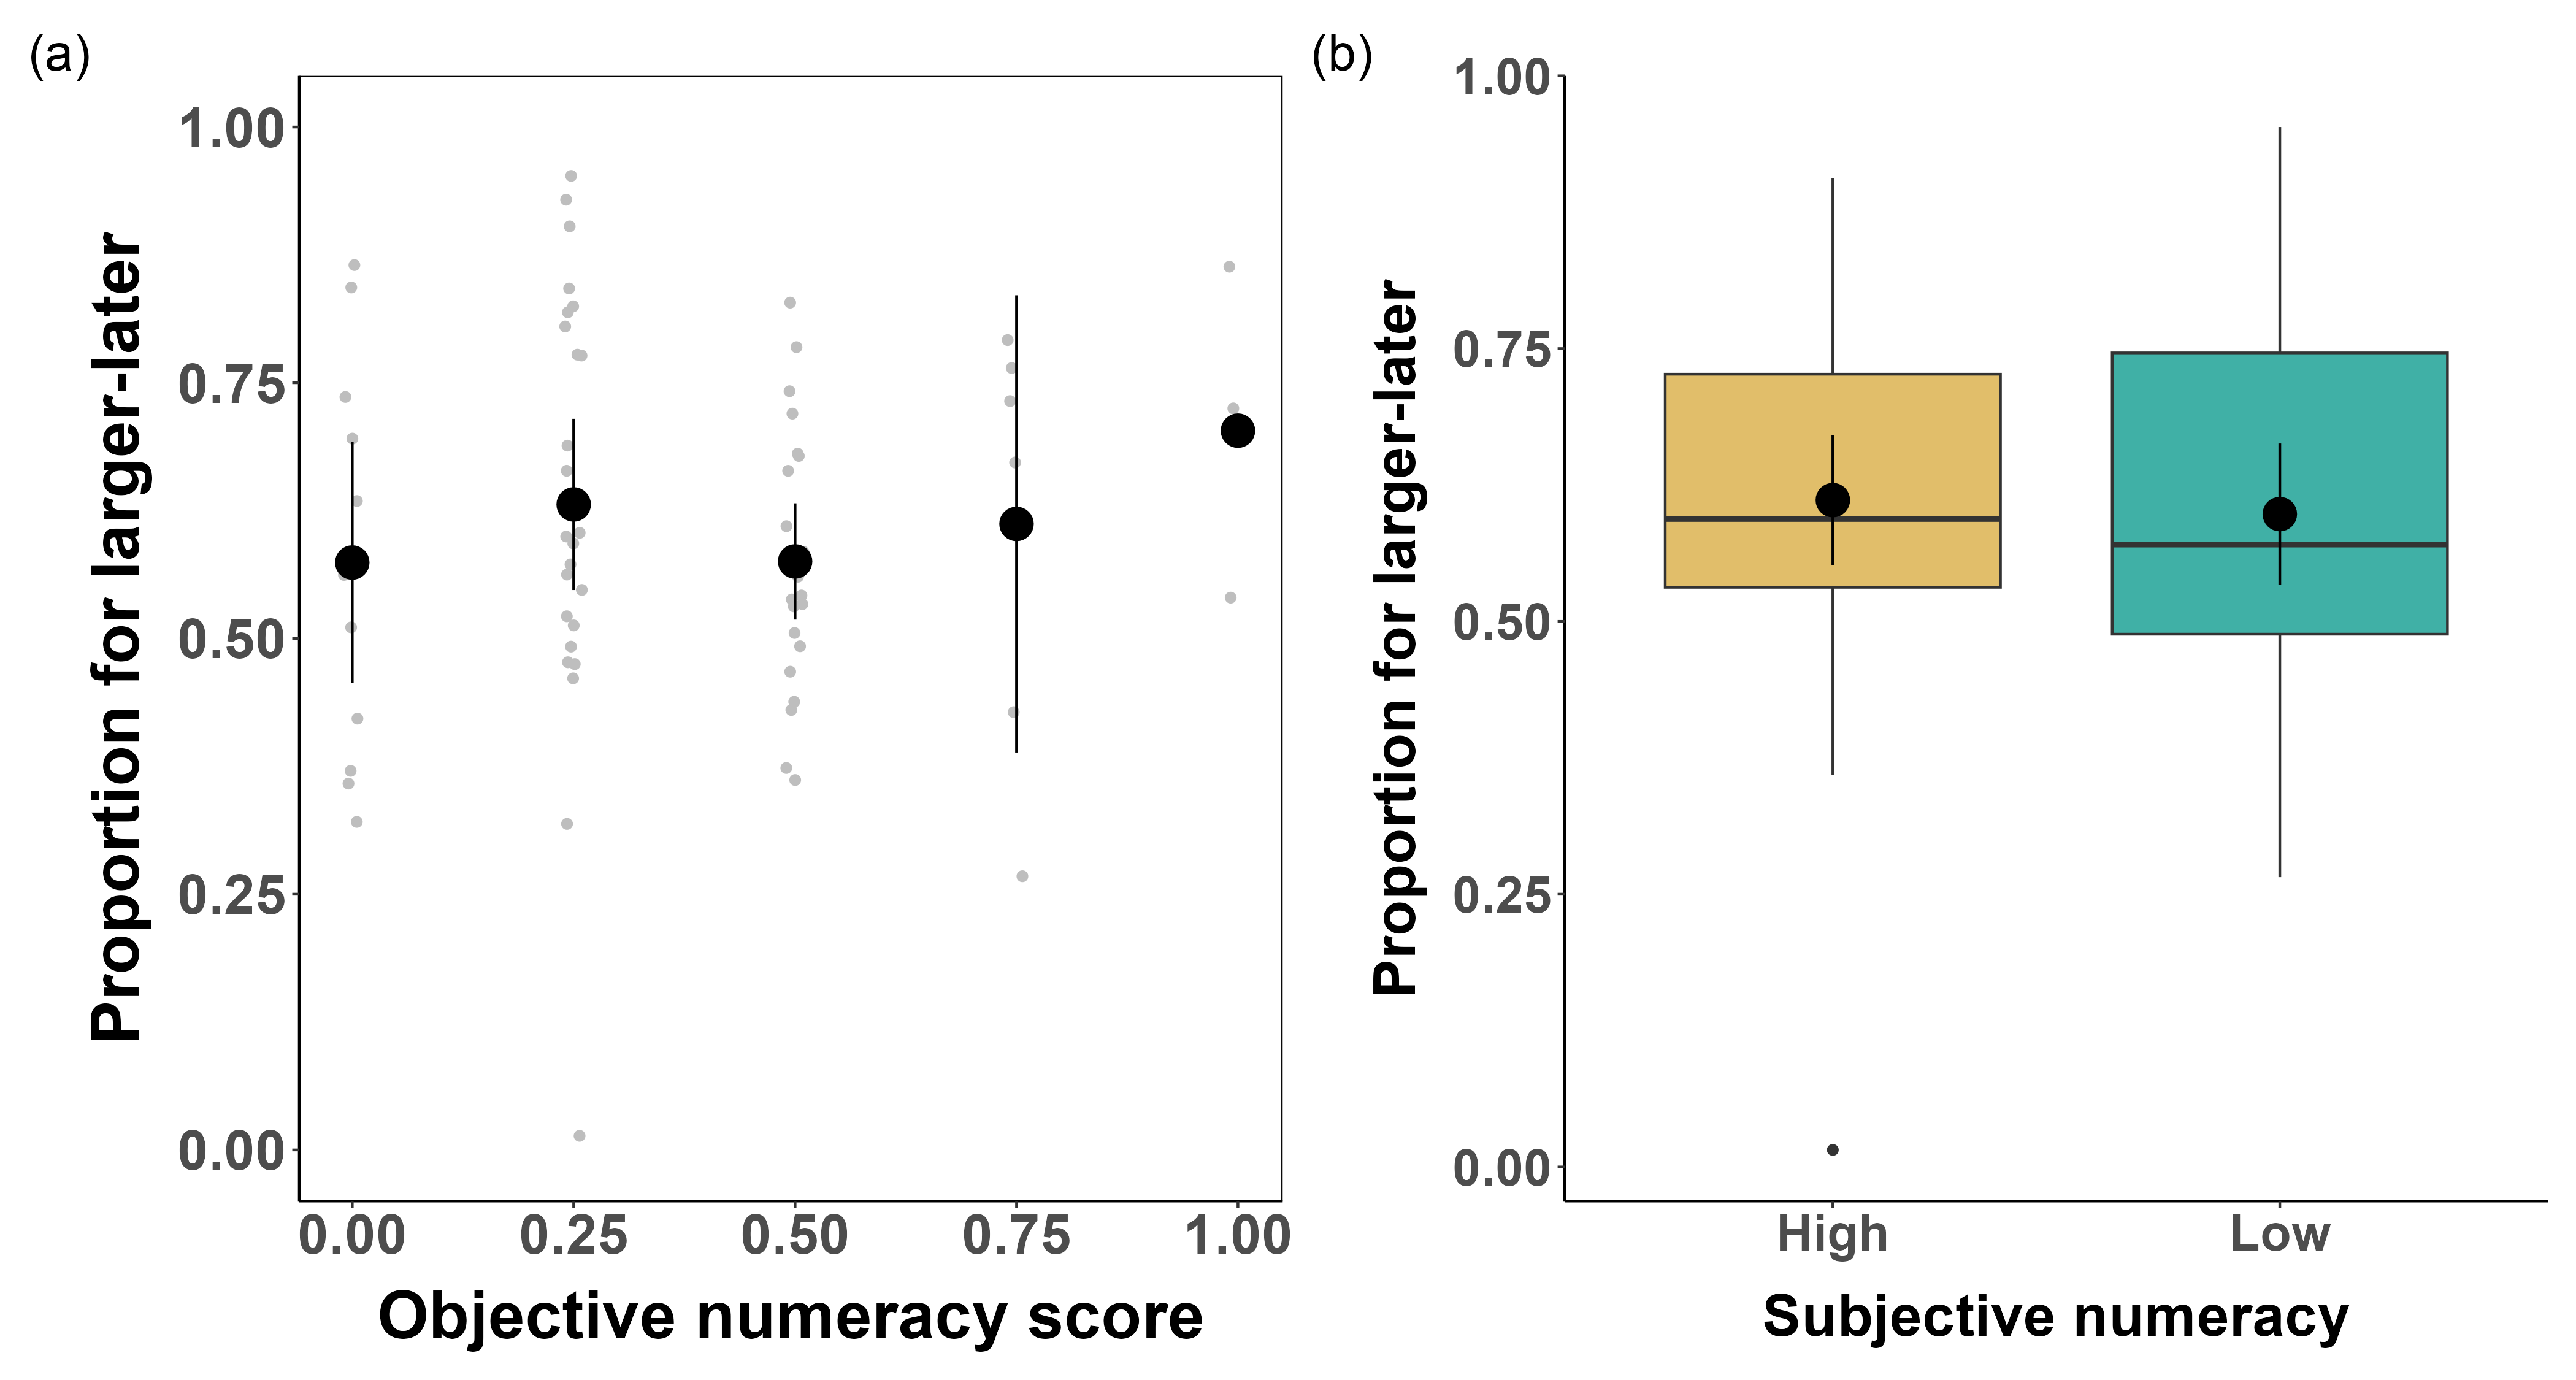
\includegraphics[width=1\linewidth]{figures/numeracy_itc_1} \caption{Proportion of larger, later options chosen in non-social intertemporal choice questions by participants according to (a) objective numeracy scores and (b) subjective numeracy levels for study 1. For boxplots, horizontal bars represent medians, boxes represent interquartile ranges (25\textsuperscript{th} - 75\textsuperscript{th} percentile), and whiskers represent 1.5 times the interquartile range. Figure used with permission under a CC-BY4.0 license: Goh \& Stevens (2022); available at \url{https://doi.org/10.31234/osf.io/xz68b}}\label{fig:numeracyitc1}
\end{figure}



\begin{figure}

{\centering 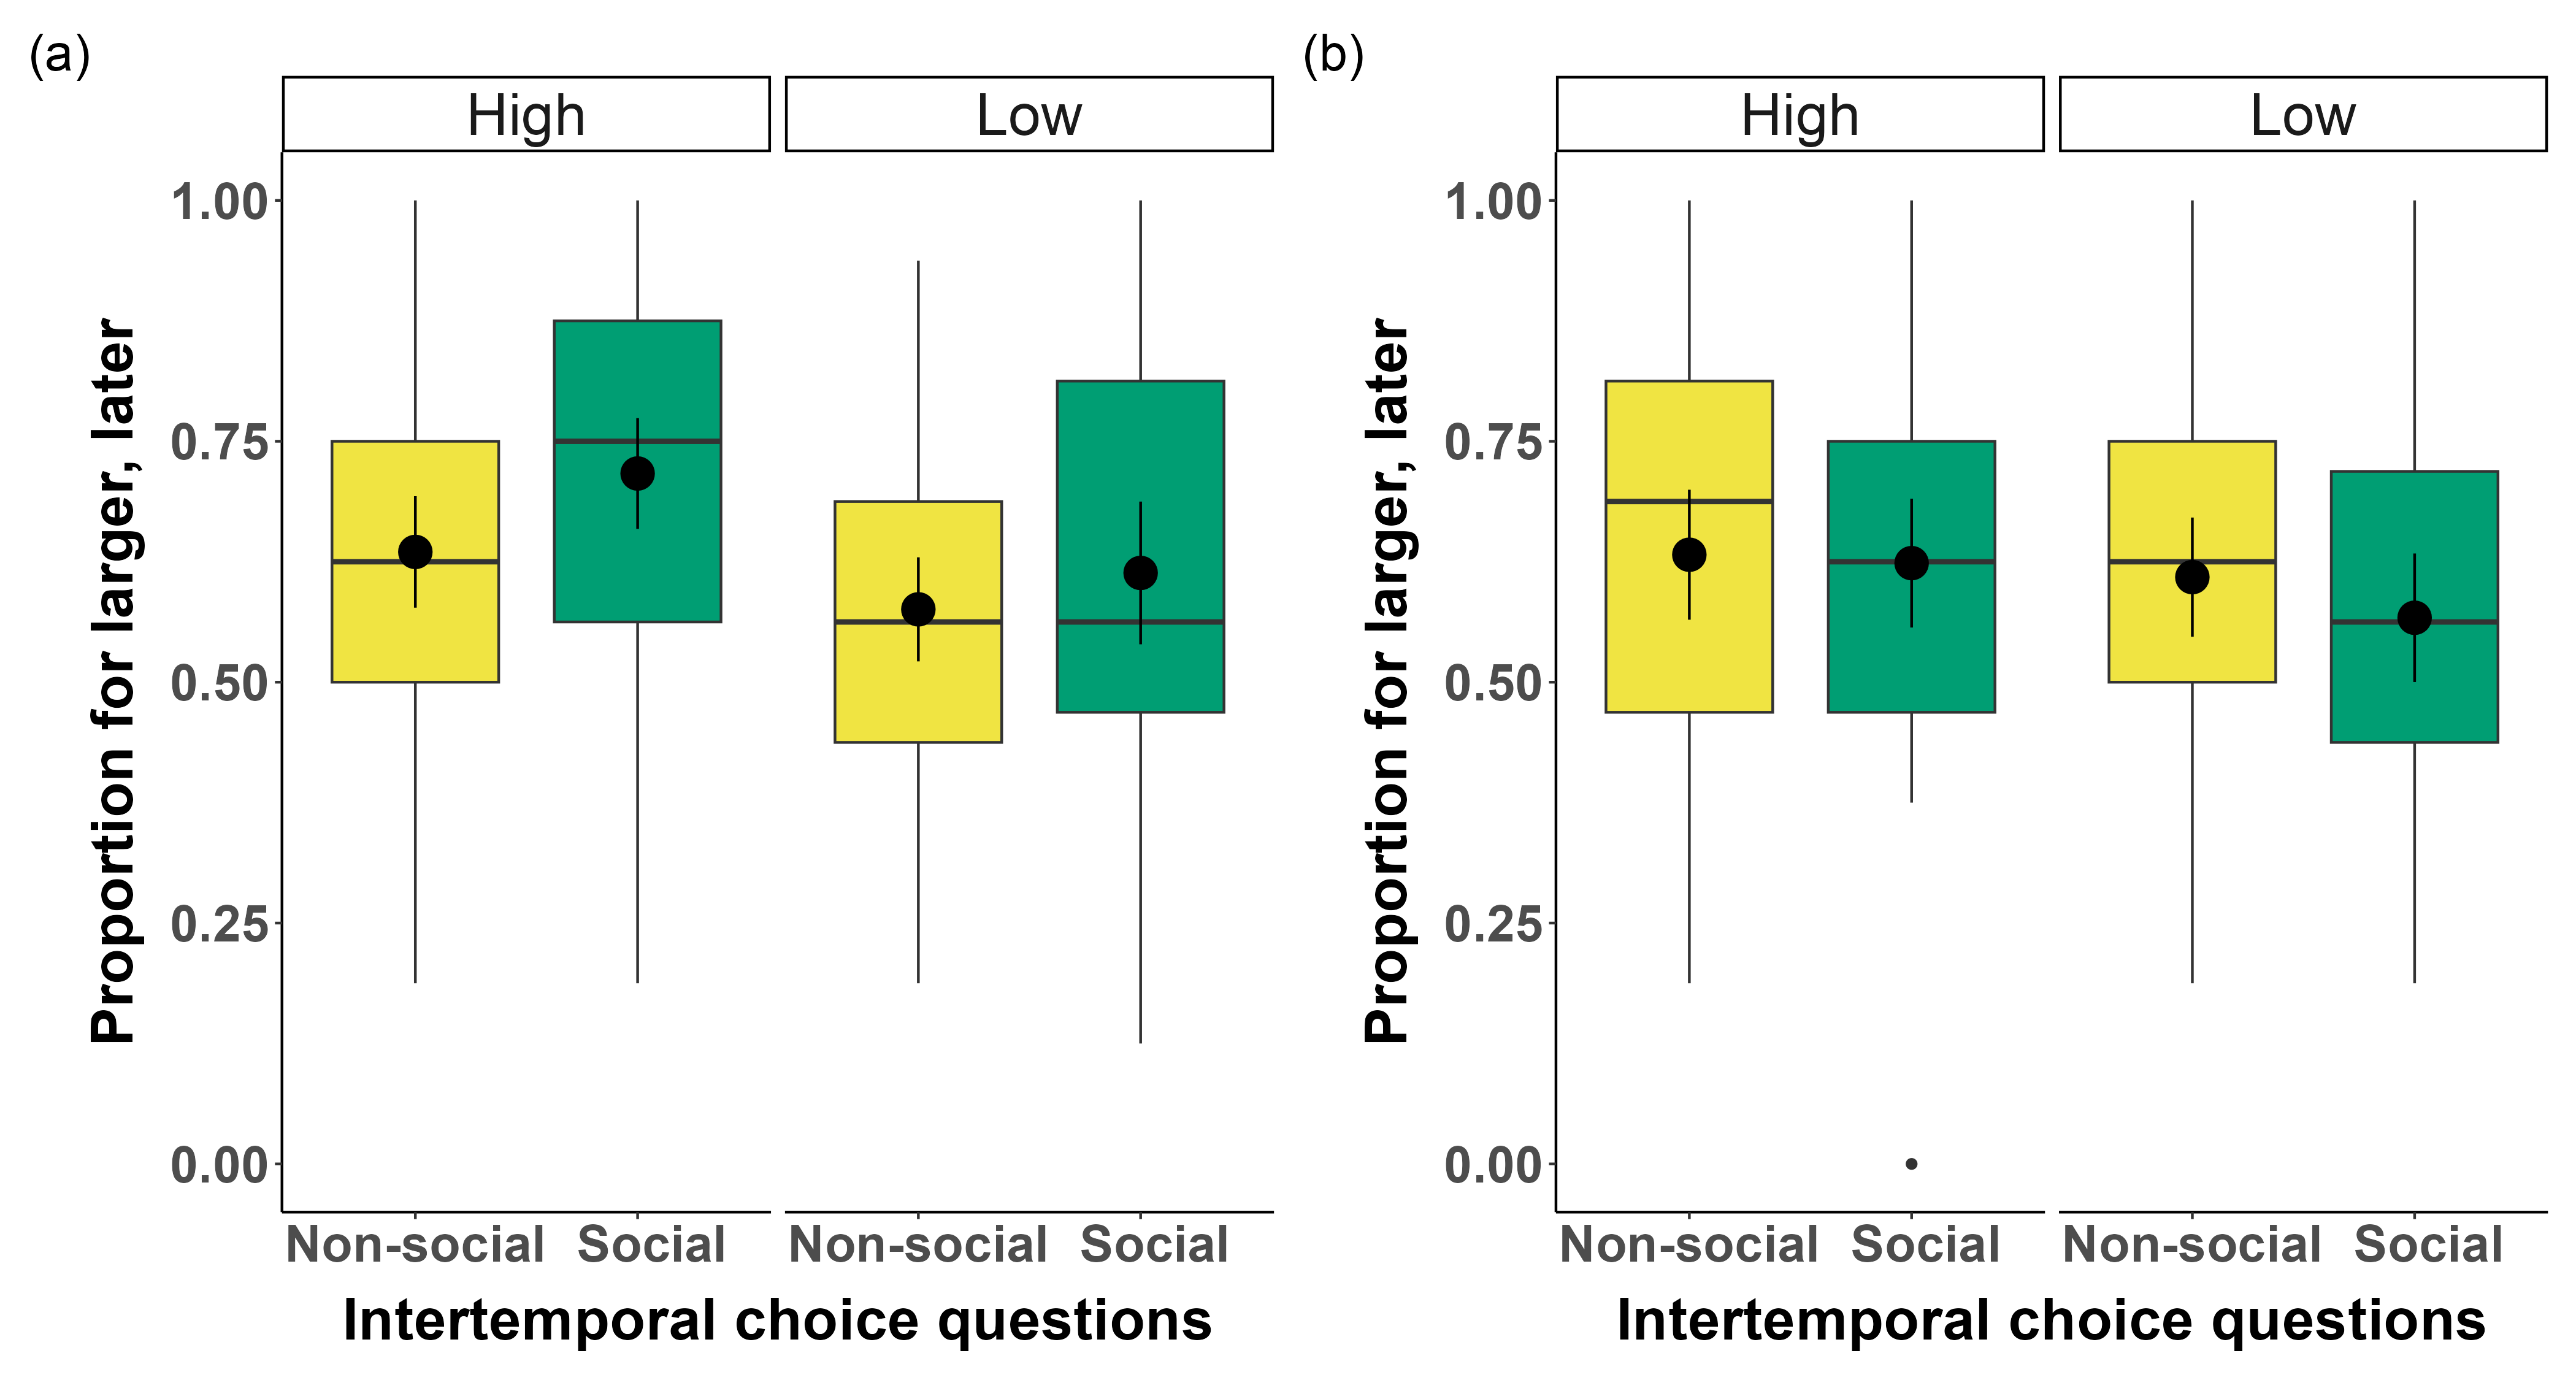
\includegraphics[width=1\linewidth]{figures/suggestibility_itc_2} 

}

\caption{Proportion of participant choices for the larger, later option for the (a) amount-focused and (b) delay-focused social information conditions for study 2. The left panels represent participant choices for the larger, later option for non-social compared to social intertemporal choice questions for those in the high suggestibility group while the right panels represent the comparison of these choices for participants in the low suggestibility group. Dots and error bars represent mean values and 95\% within-subject confidence intervals respectively. For boxplots, horizontal bars represent medians, boxes represent interquartile ranges (25\textsuperscript{th} - 75\textsuperscript{th} percentile), and whiskers represent 1.5 times the interquartile range. Figure used with permission under a CC-BY4.0 license: Goh \& Stevens (2022); available at \url{https://doi.org/10.31234/osf.io/xz68b}}\label{fig:suggestibility2}
\end{figure}



\begin{figure}
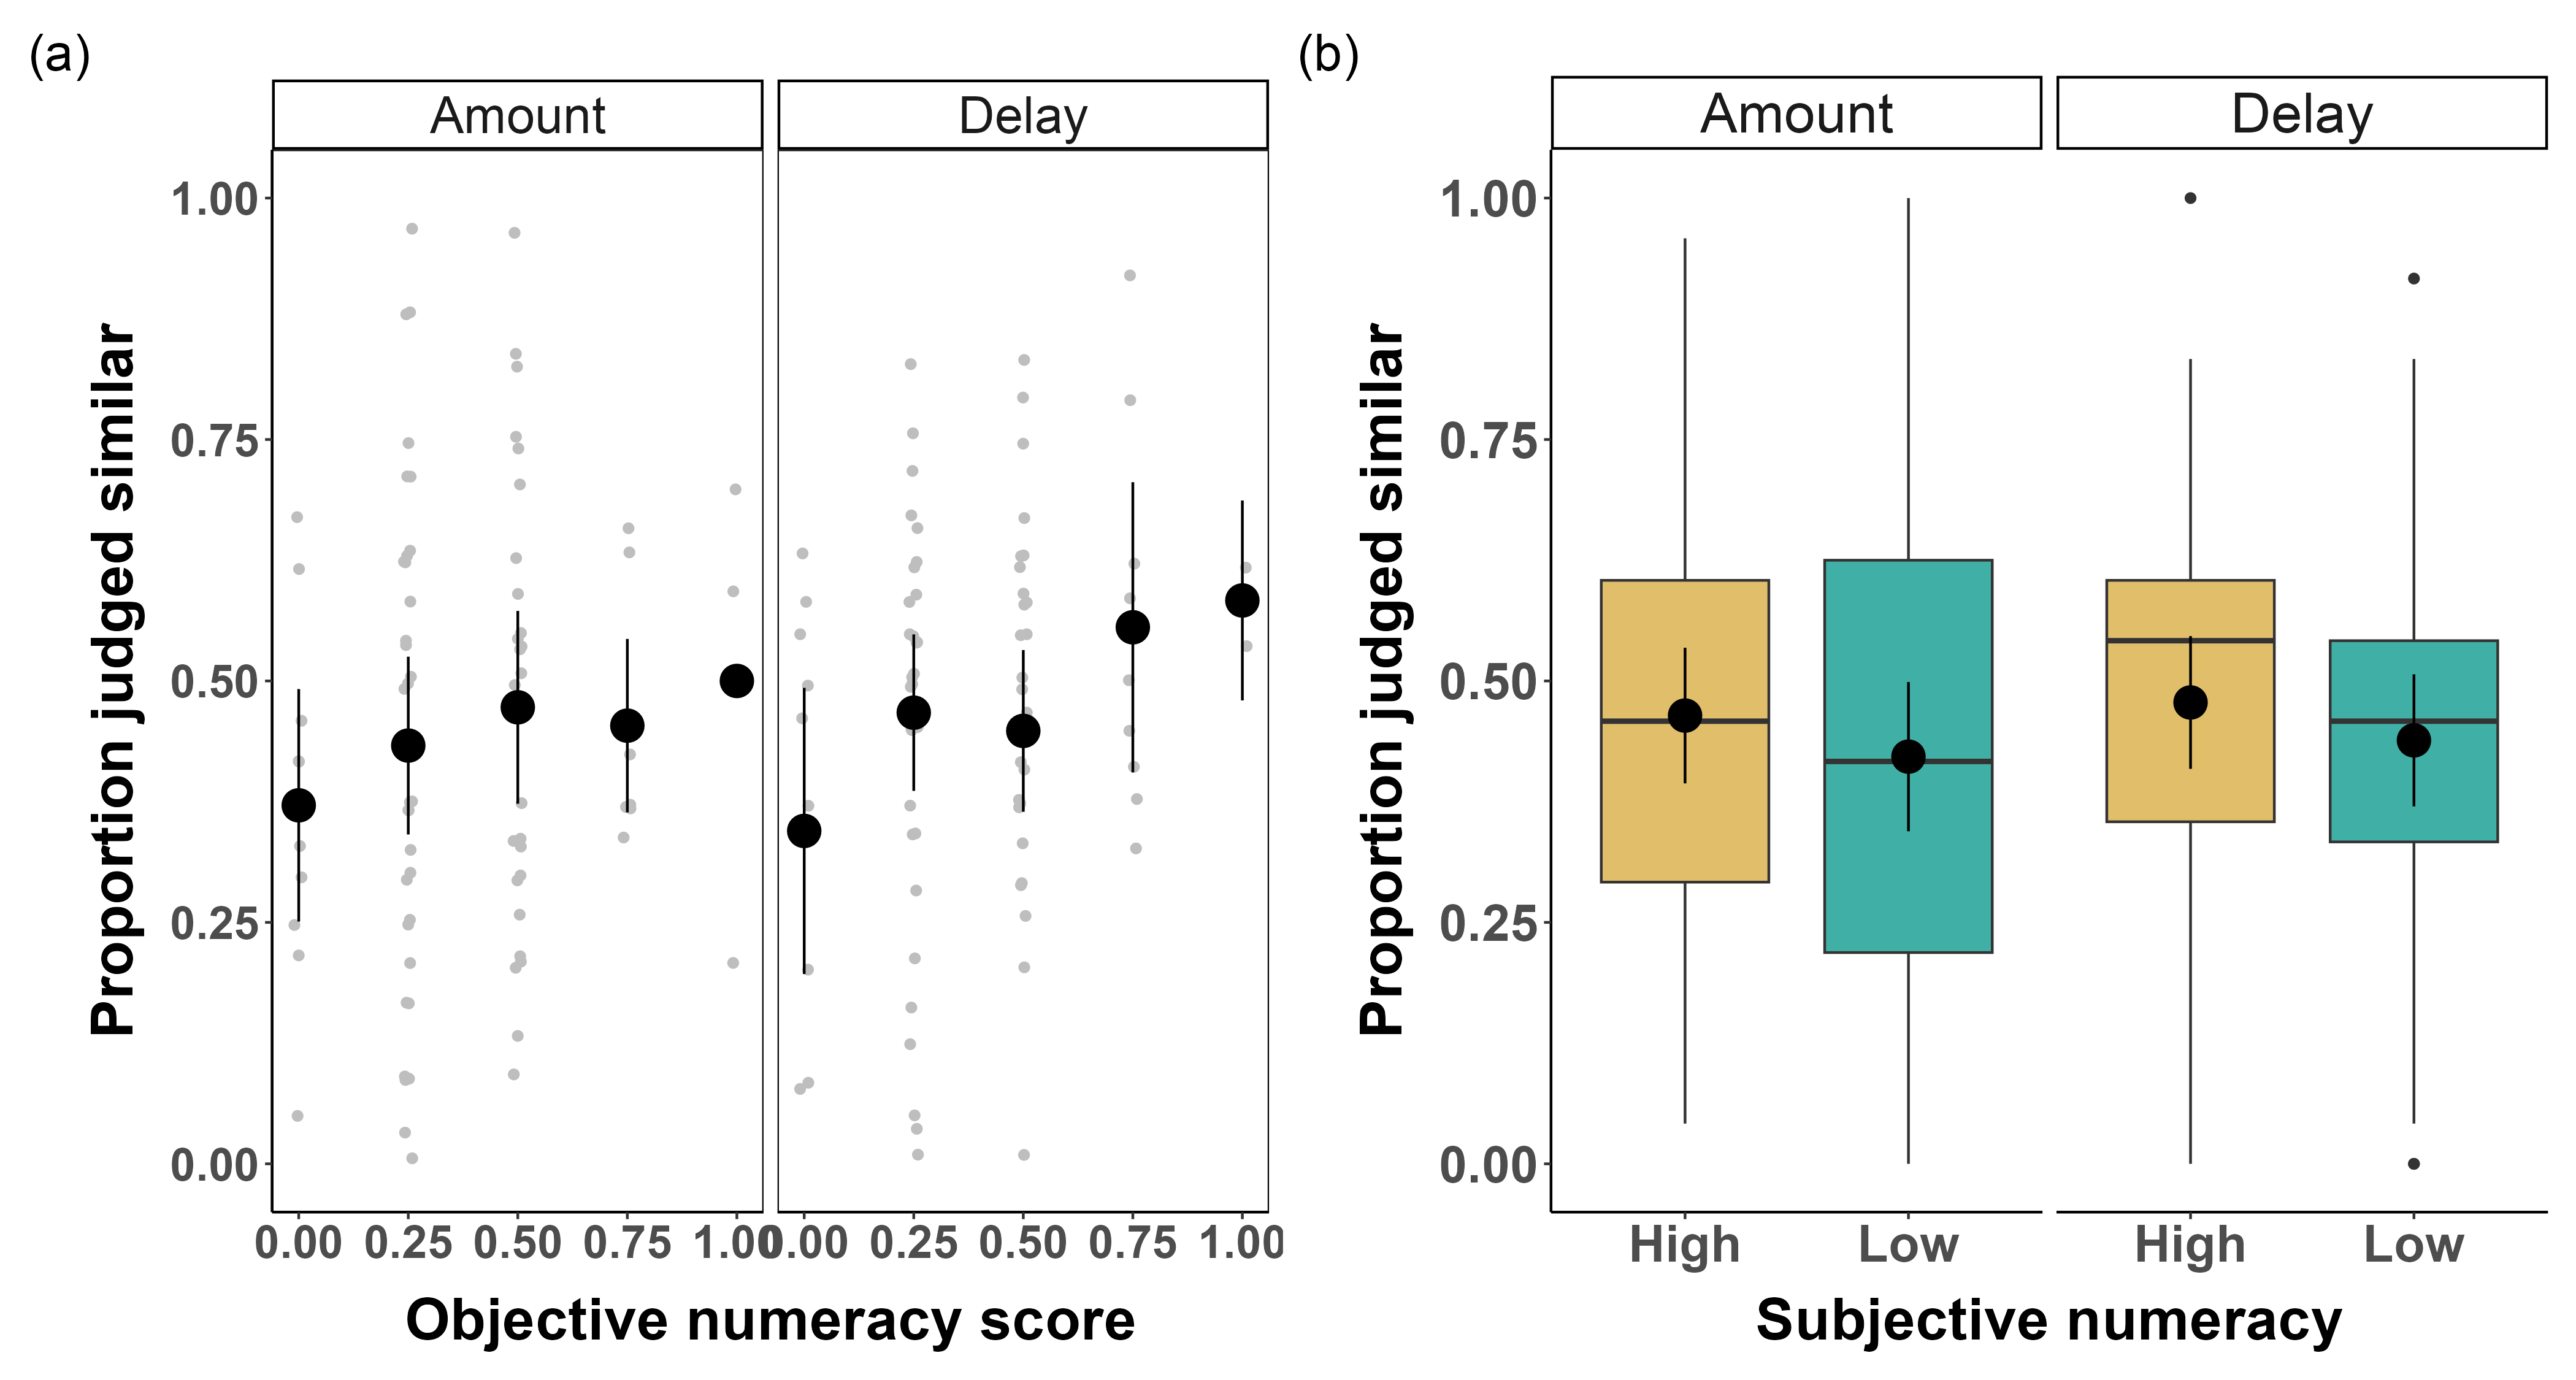
\includegraphics[width=1\linewidth]{figures/numeracy_judgments_2} \caption{Proportion of number pairs judged similar by participants according to (a) objective numeracy scores and (b) subjective numeracy levels for study 2. The left panels represent judgments in the amount similarity judgment task and the right panels represent judgments in the delay similarity judgment task. Dots and error bars represent mean values and 95\% within-subject confidence intervals respectively. For boxplots, horizontal bars represent medians, boxes represent interquartile ranges (25\textsuperscript{th} - 75\textsuperscript{th} percentile), and whiskers represent 1.5 times the interquartile range. Figure used with permission under a CC-BY4.0 license: Goh \& Stevens (2022); available at \url{https://doi.org/10.31234/osf.io/xz68b}}\label{fig:numeracyjudgments2}
\end{figure}



\begin{figure}
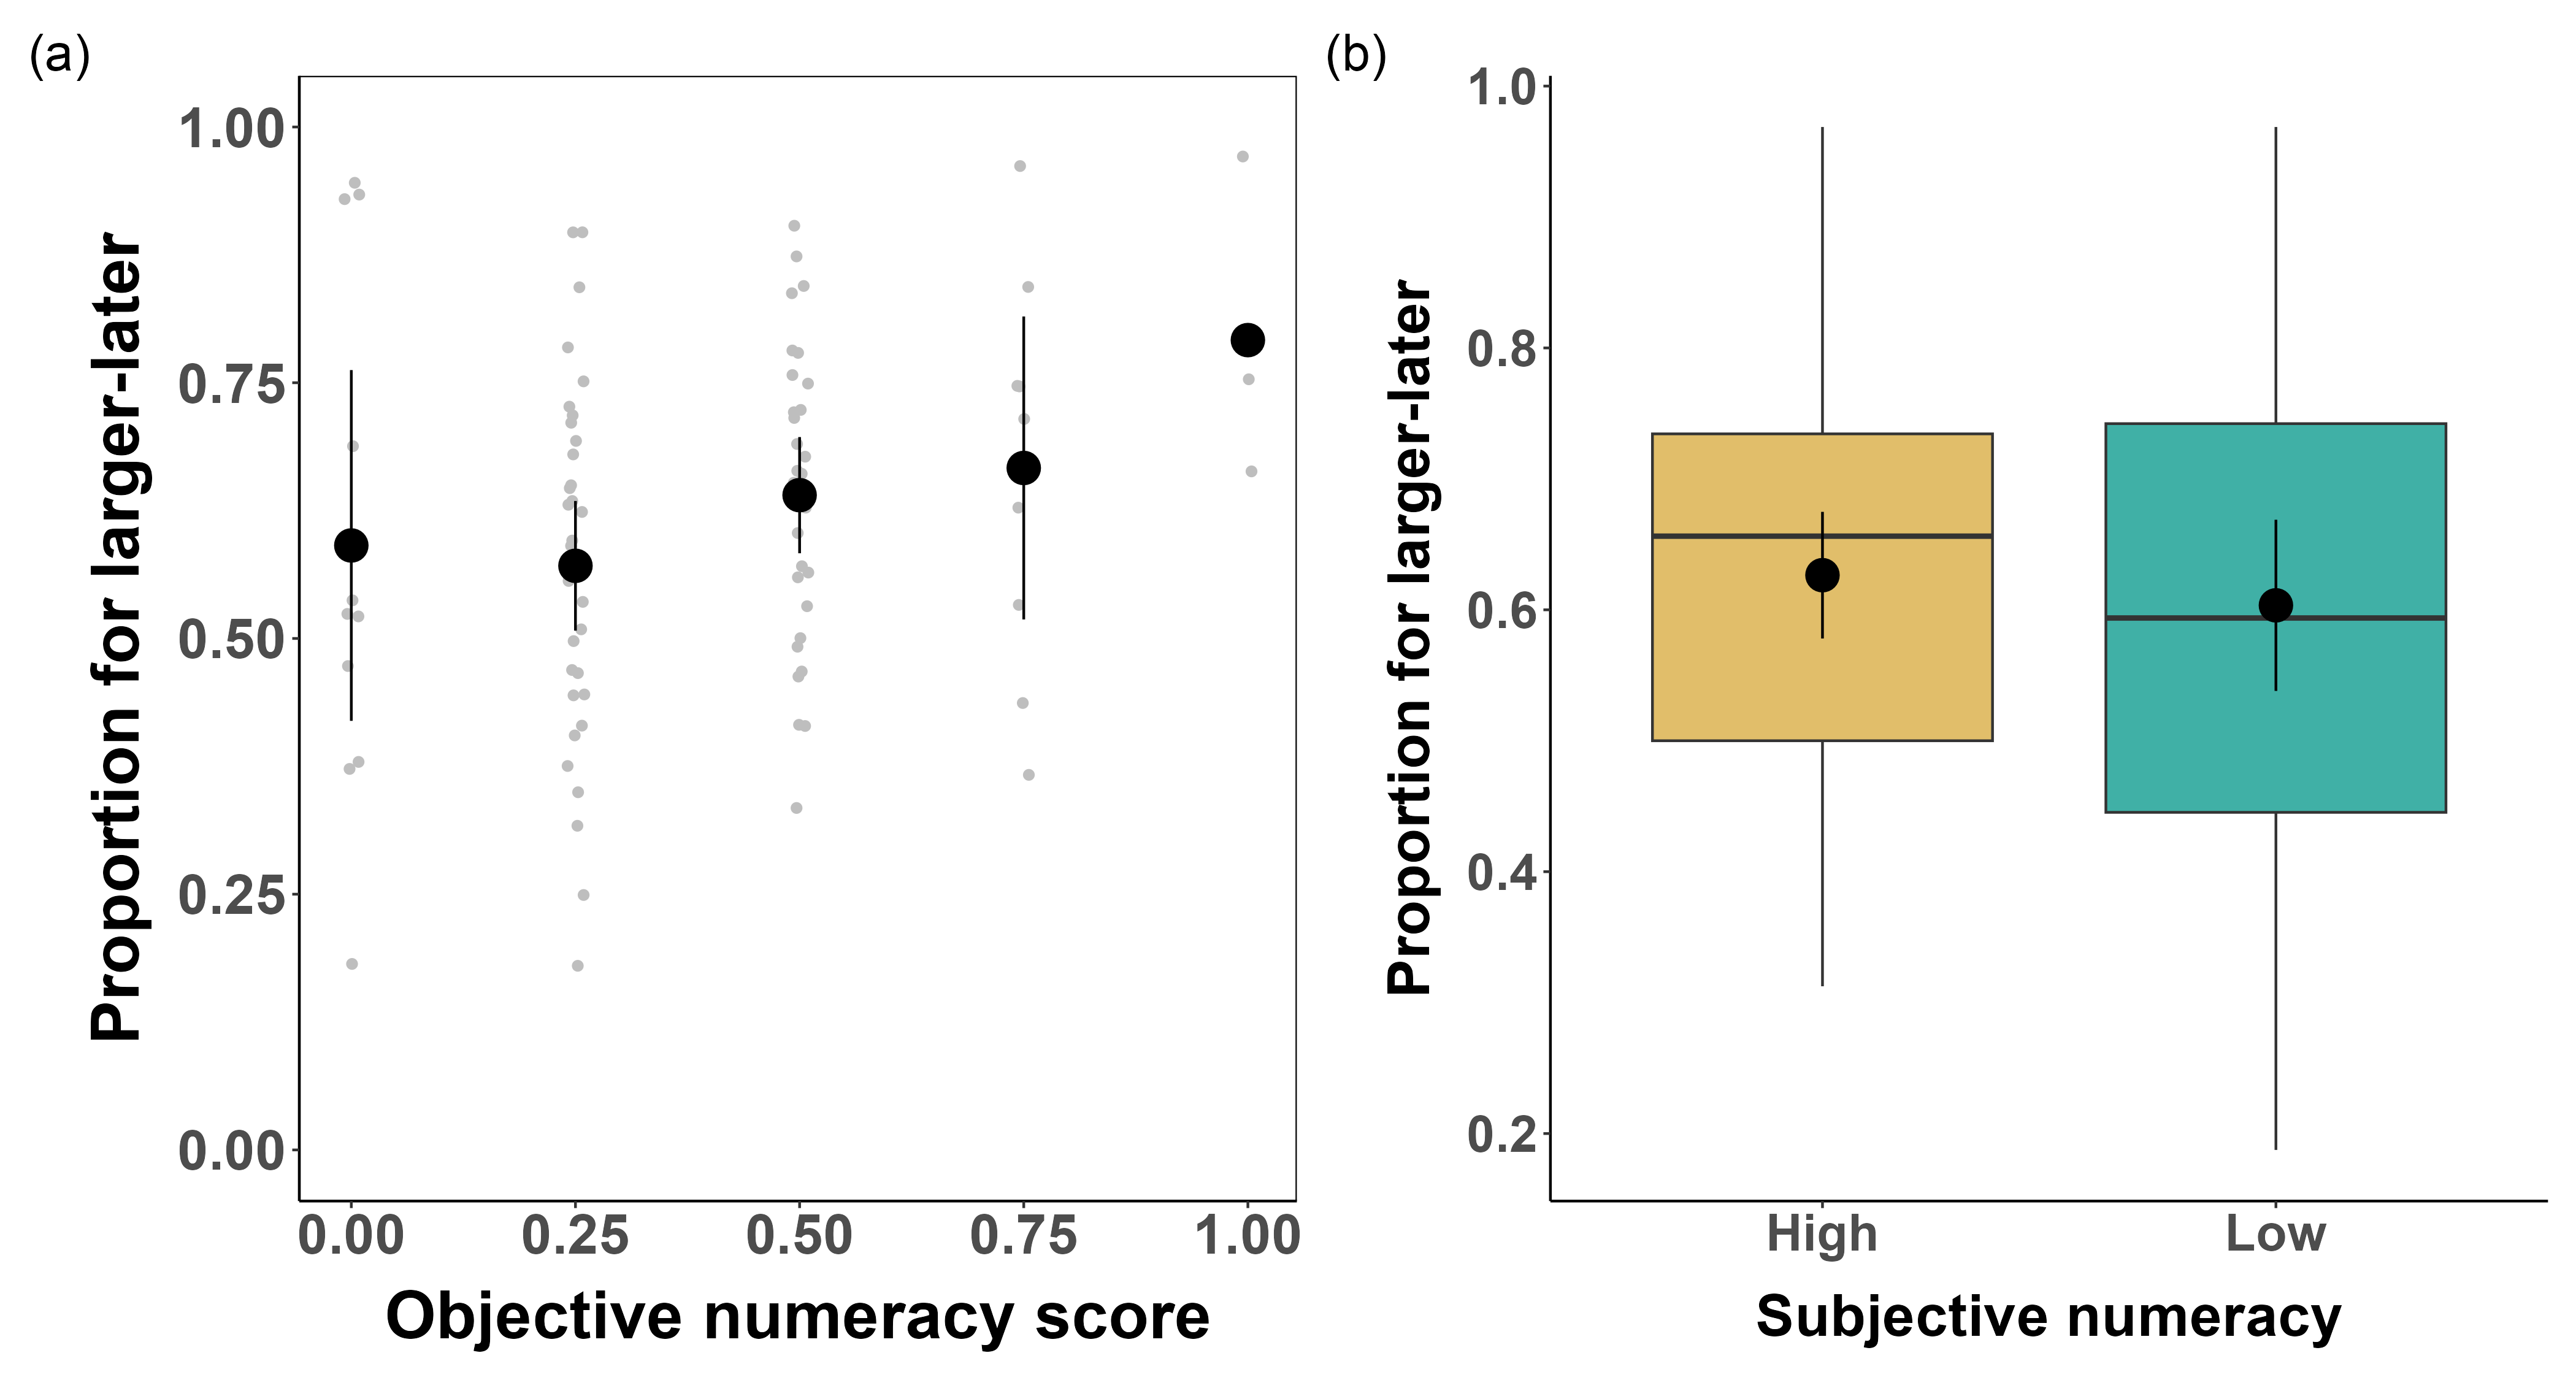
\includegraphics[width=1\linewidth]{figures/numeracy_itc_2} \caption{Proportion of larger, later options chosen in non-social intertemporal choice questions by participants according to (a) objective numeracy scores and (b) subjective numeracy levels for study 2. For boxplots, horizontal bars represent medians, boxes represent interquartile ranges (25\textsuperscript{th} - 75\textsuperscript{th} percentile), and whiskers represent 1.5 times the interquartile range. Figure used with permission under a CC-BY4.0 license: Goh \& Stevens (2022); available at \url{https://doi.org/10.31234/osf.io/xz68b}}\label{fig:numeracyitc2}
\end{figure}


\end{document}
